\section{Thiết kế giao thức}

\subsection{Lực chọn thiết kế}
Ứng dụng dùng 2 kênh có vai trò khác nhau:
\begin{itemize}
    \item TCP/TLS cho xác thực, quản lý phiên và chat. Luồng byte có thứ tự và tin cậy của TCP phù hợp với các thông điệp điều khiển ngắn.
    \item UDP cho truyền file. Độ tin cậy (xác nhận, gửi lại, kiểm tra toàn vẹn) được cài đặt ở tầng ứng dụng.
\end{itemize}

File không đi trực tiếp giữa hai client mà đi qua một UDP relay theo phiên. Relay chuyển tiếp dữ liệu nhưng không lưu nội dung file. Nhờ vậy client không cần tự dò tìm địa chỉ của người nhận, và relay có thể kiểm tra từng gói theo phiên đã xác thực.

Server TCP chỉ ghi nhận cổng TCP của client, mà cổng này không cho biết socket UDP nhận file nằm ở đâu. Vì vậy mỗi client phải đăng ký điểm cuối UDP của mình với relay bằng một thủ tục có thử thách (challenge), mô tả ở mục 3.3.

Toàn bộ \texttt{OFFER}, \texttt{ACCEPT}, \texttt{DATA}, \texttt{ACK}, \texttt{FIN} và \texttt{COMPLETE} của file đi qua UDP. Chúng không phải là action TCP và không đi qua \texttt{MessageRouter} của server.

\subsection{Giao thúc điều kiển TCP}
Mặc định server dùng cổng TCP 5000 và relay dùng cổng UDP 5001, cả hai đều cấu hình được. Sau handshake \texttt{HELLO2}/\texttt{WELCOME2} trong TLS, mỗi thông điệp là một đối tượng JSON UTF-8 kết thúc bằng LF; ký tự xuống dòng bên trong nội dung phải được escape. Bên nhận phải đệm dữ liệu và tách từng dòng hoàn chỉnh, vì một lần recv có thể chứa nửa thông điệp hoặc nhiều thông điệp.

Ba loại thông điệp được phân biệt bằng trường định danh:

\begin{table}[H]
    \centering
    \renewcommand{\arraystretch}{1.3}

    \begin{tabular}{@{} l l l @{}}
        \toprule
        \textbf{Loại} & \textbf{Trường} & \textbf{Hướng} \\
        \midrule
        Yêu cầu                  & \texttt{action} & Client $\rightarrow$ Server \\
        Phản hồi                 & \texttt{status} & Server $\rightarrow$ Client \\
        Sự kiện chat bất đồng bộ & \texttt{type}   & Server $\rightarrow$ Client \\
        \bottomrule
    \end{tabular}
\end{table}

Mã trạng thái là chuỗi chữ hoa, phân biệt hoa thường, không phải mã HTTP. Danh sách action và status đầy đủ nằm ở mục 4.4. Ví dụ một phiên trao đổi (dạng logic, trước lớp mã hóa chat ở mục 6):

\begin{lstlisting}[style=json]
    {"action":"REGISTER","username":"alice","password":"example-only"}
    {"status":"REGISTER_SUCCESS"}

    {"action":"LOGIN","username":"alice","password":"example-only"}
    {"status":"LOGIN_SUCCESS"}

    {"action":"UNICAST","recipient":"bob","message":"Hello"}
    {"type":"UNICAST","sender":"alice","recipient":"bob","message":"Hello"}
    {"status":"UNICAST_SUCCESS"}

    {"action":"LIST_ONLINE"}
    {"status":"LIST_ONLINE_SUCCESS","users":["alice","bob"]}
\end{lstlisting}

Dòng thứ sáu là sự kiện server gửi cho bob, các dòng còn lại là phản hồi cho alice. Do giao thức không có mã yêu cầu, một kết nối chỉ có một yêu cầu chờ phản hồi tại một thời điểm, và bên đọc phải tách \texttt{status} khỏi \texttt{type} vì sự kiện có thể xen giữa các phản hồi.


\begin{figure}[H]
    \centering
    \begin{tikzpicture}[
        >=Stealth,
        scale=0.95,
        transform shape,
        state/.style={
            draw=black!65,
            rounded corners=3pt,
            minimum width=2.4cm,
            minimum height=0.65cm,
            align=center,
            font=\small
        },
        transition/.style={
            ->,
            thick,
            draw=black!55
        },
        event/.style={
            font=\footnotesize,
            align=center,
            fill=white,
            inner sep=2pt
        }
    ]

    % States
    \node[state] (disconnected) at (0,0) {Disconnected};
    \node[state] (handshake) at (-2.2,-1.8) {Handshake};
    \node[state] (unauth) at (-1.5,-3.5) {Unauthenticated};
    \node[state] (auth) at (-0.7,-5.2) {Authenticated};
    \node[state] (udp) at (-0.7,-6.7) {UdpUnbound};
    \node[state] (ready) at (-0.1,-8.4) {Ready};

    % Initial state
    \fill (0,0.9) circle (2pt);
    \draw[transition] (0,0.9) -- (disconnected.north);

    % Disconnected -> Handshake
    \draw[transition]
        (disconnected.west)
        to[out=210,in=30]
        node[event, pos=0.48, above left]
        {TLS connect, HELLO2}
        (handshake.north east);

    % Handshake -> Disconnected
    \draw[transition]
        (handshake.north west)
        to[out=150,in=225]
        node[event, pos=0.45, left]
        {timeout / invalid handshake}
        (disconnected.south west);

    % Handshake -> Unauthenticated
    \draw[transition]
        (handshake.south)
        -- node[event, midway, left] {WELCOME2}
        (unauth.north);

    % Unauthenticated -> Authenticated
    \draw[transition]
        (unauth.south)
        to[out=270,in=120]
        node[event, midway, left] {LOGIN\_SUCCESS}
        (auth.north);

    % Unauthenticated -> Disconnected
    \draw[transition]
        (unauth.east)
        .. controls (1.7,-3.1) and (1.7,-0.7)
        .. node[event, pos=0.55, right]
        {idle timeout / disconnect}
        (disconnected.south);

    % Authenticated -> Disconnected
    \draw[transition]
        (auth.east)
        .. controls (2.6,-4.8) and (2.6,-1.0)
        .. node[event, pos=0.48, right]
        {idle timeout / disconnect}
        (disconnected.east);

    % Authenticated -> UdpUnbound
    \draw[transition]
        (auth.south)
        -- node[event, midway, left]
        {FILE\_SESSION (ticket issued)}
        (udp.north);

    % UdpUnbound -> Ready
    \draw[transition]
        (udp.south)
        -- node[event, midway, left]
        {BIND / CHALLENGE /\\ PROVE / BOUND}
        (ready.north);

    % Ready -> Disconnected
    \draw[transition]
        (ready.east)
        .. controls (4.0,-7.9) and (4.0,-0.5)
        .. node[event, pos=0.48, right]
        {logout / disconnect (ticket\\ revoked)}
        (disconnected.east);

    \end{tikzpicture}

    \caption{State machine của kết nối client}
\end{figure}

\subsection{Giao thức file trên UDP}
Mỗi datagram là một gói hoàn chỉnh, các số nguyên theo thứ tự byte mạng (network byte order). Phần đầu (header) dài 44 byte:


\begin{table}[H]
    \centering
    \small
    \renewcommand{\arraystretch}{1.3}

    \begin{tabularx}{\textwidth}{
        @{}
        >{\raggedleft\arraybackslash}p{1cm}
        >{\raggedleft\arraybackslash}p{1cm}
        >{\raggedright\arraybackslash}X
        @{}
    }
        \toprule
        \textbf{Offset} & \textbf{Byte} & \textbf{Trường} \\
        \midrule

        0  & 4  & Magic \texttt{P1FT} \\

        4  & 1  & Phiên bản giao thức (hiện là 2) \\

        5  & 1  & Loại thông điệp \\

        6  & 16 & UUID phiên của client trên chặng relay này \\

        22 & 16 & UUID của lượt truyền; toàn số 0 với thông điệp cấp phiên \\

        38 & 4  & Số thứ tự chunk bắt đầu từ 0; bằng 0 với thông điệp điều khiển \\

        42 & 2  & Độ dài payload đã mã hóa \\

        \bottomrule
    \end{tabularx}
\end{table}

\vspace{-1.8em}
Sau header là phần thân: \texttt{nonce} 12 byte, dữ liệu mã hóa (0 đến 996 byte), thẻ GCM 16 byte và thẻ HMAC 16 byte. Mỗi chunk file mang tối đa 996 byte dữ liệu gốc, nên một datagram DATA dài tối đa 1.084 byte, còn gói điều khiển rỗng chỉ 88 byte. Kích thước này được chọn thận trọng để giảm nguy cơ phân mảnh IP trên mạng LAN thông thường; nó không thay thế việc dò MTU của đường truyền. Ý nghĩa của nonce, thẻ GCM và HMAC được giải thích ở mục 6.

Các loại thông điệp:

\begin{table}[H]
    \centering
    \small
    \renewcommand{\arraystretch}{1.3}

    \begin{tabularx}{\textwidth}{
        @{}
        >{\raggedleft\arraybackslash}p{1.2cm}
        >{\centering\arraybackslash}p{2.2cm}
        >{\raggedright\arraybackslash}X
        @{}
    }
        \toprule
        \textbf{Giá trị} & \textbf{Loại} & \textbf{Ý nghĩa} \\
        \midrule

        1  & \texttt{BIND}      & Yêu cầu đăng ký điểm cuối UDP \\
        2  & \texttt{BOUND}     & Xác nhận đã đăng ký điểm cuối \\
        3  & \texttt{OFFER}     & Đề nghị gửi file, kèm siêu dữ liệu (metadata) JSON \\
        4  & \texttt{ACCEPT}    & Người nhận đồng ý và đã cấp phát trạng thái nhận \\
        5  & \texttt{REJECT}    & Người nhận từ chối, kèm lý do \\
        6  & \texttt{DATA}      & Một chunk dữ liệu file \\
        7  & \texttt{ACK}       & Người nhận đã ghi chunk đó \\
        8  & \texttt{FIN}       & Người gửi đã nhận ACK cho mọi chunk \\
        9  & \texttt{COMPLETE}  & Người nhận đã kiểm tra kích thước, SHA-256 và lưu file \\
        10 & \texttt{ERROR}     & Mã lỗi \\
        11 & \texttt{CANCEL}    & Hủy lượt truyền \\
        12 & \texttt{PING}      & Giữ phiên UDP \\
        13 & \texttt{PONG}      & Phản hồi PING \\
        14 & \texttt{CHALLENGE} & Số ngẫu nhiên 16 byte do relay cấp cho điểm cuối mới \\
        15 & \texttt{PROVE}     & Gửi lại số ngẫu nhiên đó, kèm thẻ xác thực \\

        \bottomrule
    \end{tabularx}
\end{table}

Siêu dữ liệu OFFER gồm: \texttt{recipient} (tên người nhận), filename (tên tệp 1 đến 128 byte UTF-8, không chứa đường dẫn hay ký tự điều khiển), \texttt{size} (0 đến 268.435.456 byte, tức tối đa 256 MiB), \texttt{sha256} (64 ký tự hex thường), \texttt{chunk\_size} và texttt{total\_chunks}. Relay tự thêm trường \texttt{sender} từ phiên đã xác thực, không bao giờ tin giá trị client tự khai, và từ chối OFFER có kích thước hoặc số chunk không nhất quán. File rỗng không có chunk nào và đi thẳng từ ACCEPT sang FIN.

Đăng ký điểm cuối UDP. Trước khi dùng UDP, client phải có ticket do server cấp qua \texttt{FILE\_SESSION}. Sau đó client gửi BIND, relay trả CHALLENGE chứa số ngẫu nhiên 16 byte gắn với điểm cuối đó và có hạn 5 giây, client trả lại số này trong PROVE có xác thực, và chỉ khi đó relay mới gửi BOUND. Một bằng chứng cũ bị bắt lại không thể dùng để chuyển điểm cuối sang địa chỉ khác. Khi đăng ký lại từ điểm cuối mới, các lượt truyền đang chạy bị hủy chứ không được tiếp tục.

Các mã ERROR đang dùng: \texttt{INVALID\_METADATA}, \texttt{TRANSFER\_ID\_CONFLICT}, \texttt{SELF\_TRANSFER}, \texttt{RECIPIENT\_OFFLINE}, \texttt{TRANSFER\_LIMIT}, \texttt{\small{PEER}\_DISCONECTED}, \texttt{ENDPOINT\_CH\small{AN}GED}, \texttt{TRANSFER\_EXPIRED}, \texttt{DISK\_EROR}, \texttt{INTEGRITY\_OR\_DISK\_EROR} và \texttt{CANCLED}. Đối với thông điệp CANCEL có thể mang 2 mã \texttt{CLIENT\_CLOSED} hoặc \texttt{SENDER\_FAILED}, còn REJECT mặc định mang \texttt{REJECTED}. Các lỗi hết hạn hoặc hết số lần gửi lại chỉ sinh ra sự kiện \texttt{file\_failed} cục bộ, không phải mã trạng thái TCP mới.

\subsection{Máy trạng thái}
Mỗi lượt truyền file có hai máy trạng thái độc lập, một ở người gửi và một ở người nhận:
\begin{itemize}
    \item Người gửi: Offering → Sending (nhận ACCEPT) → Verifying (đã được ACK mọi chunk và gửi FIN) → Complete (nhận COMPLETE). Từ chối, lỗi, hết số lần gửi lại, hết hạn hoặc hủy đều dẫn tới Failed.
    \item Người nhận: Offered → Receiving (chấp nhận và tạo file tạm) → Verifying (nhận FIN, đủ chunk) → Complete (khớp kích thước và SHA-256 thì đổi tên nguyên tử thành file chính thức). Mọi nhánh lỗi đều xóa file tạm.
\end{itemize}

Người gửi chỉ được coi là thành công sau khi nhận COMPLETE, không phải khi đã gửi xong hay đã được ACK hết chunk.
\begin{figure}[H]
    \centering
    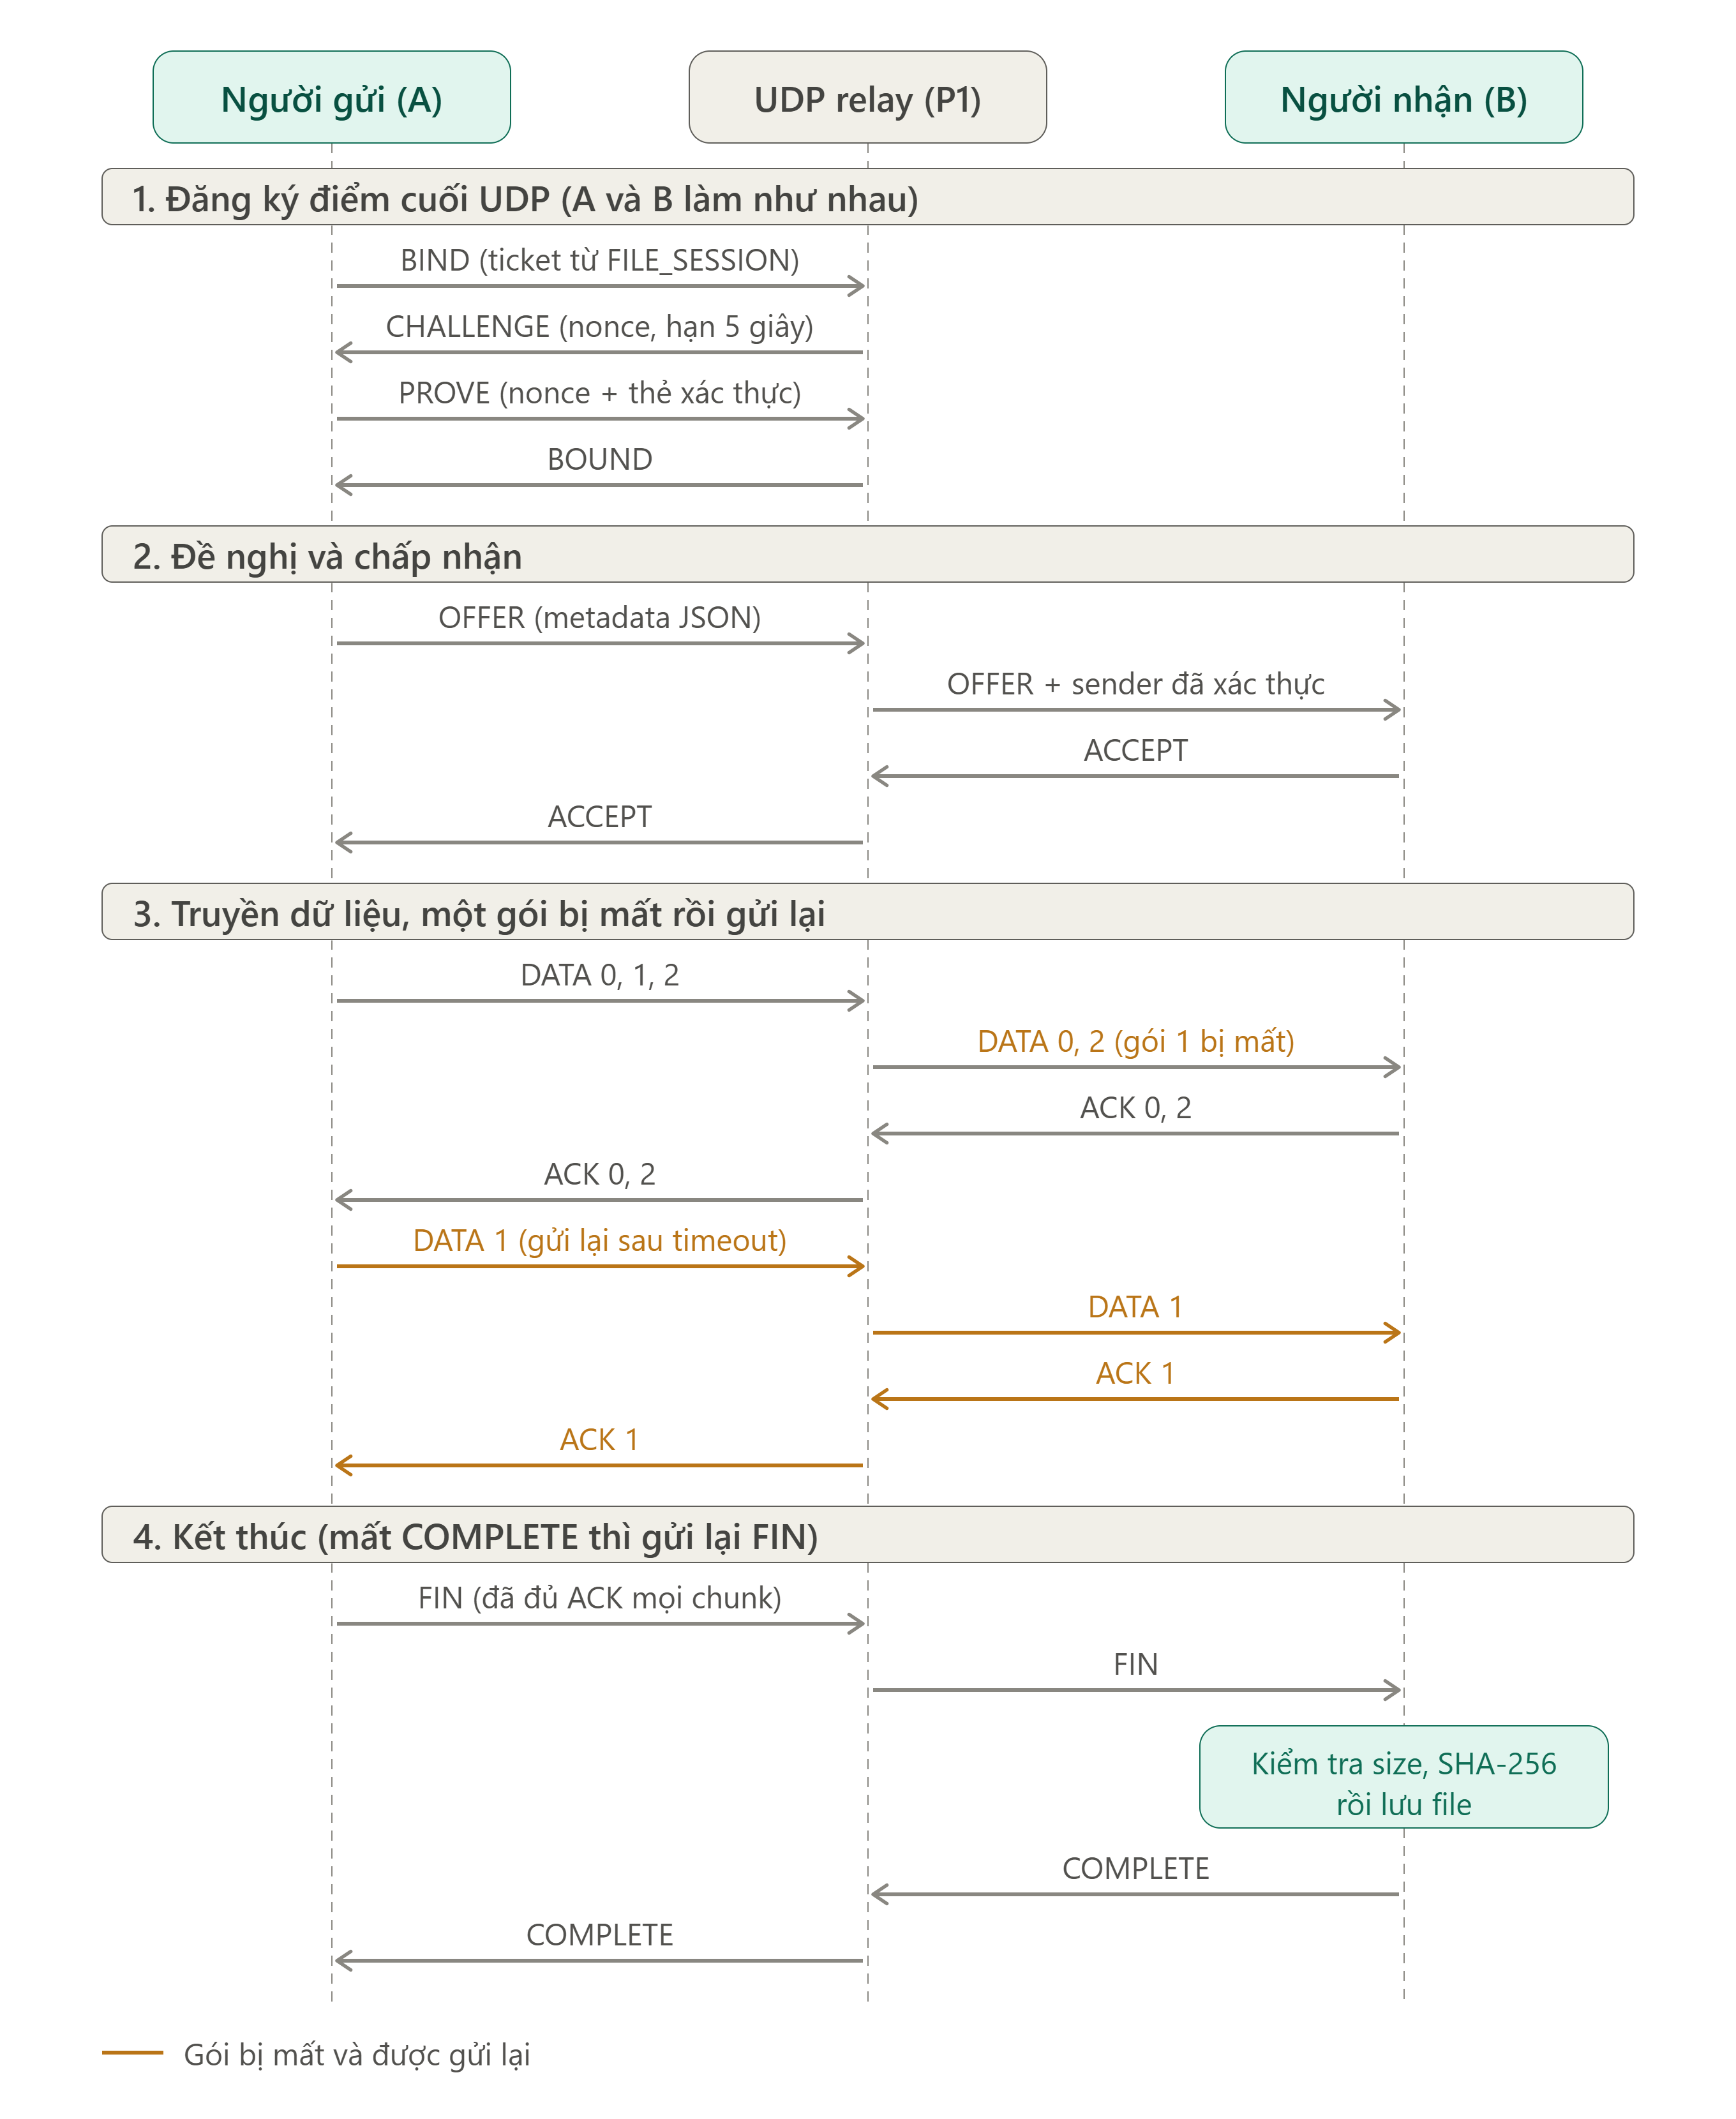
\includegraphics[width=\textwidth]{Assets/file_transfer_sequence_diagram.png}
    \caption{Trình tự truyền một file qua UDP relay}
\end{figure}